\chapter{有机金属催化：基元反应与催化循环}\label{ch:b2:catalytic-cycles}

只需几毫克钯盐，就能在烧瓶中连接两个芳香环，
而烧瓶里盛着数千克试剂：同一金属原子可以
重复完成这一工作数千次，每经一轮便回到其起始状态。
其机理由\omterm{def:b2:catalytic-cycles:cycle}{催化循环}来描述，即由几个基元反应组成的闭合序列。
基元反应只有少数几类，每一类都以固定的方式改变
金属的氧化数、电子计数和配体数。借助
\cref{ch:b2:coordination-complexes}中的电子计数，
\omterm{def:b2:catalytic-cycles:cycle}{催化循环}便可被读懂、核对，有时还可预测。

\begin{recall}
\Cref{ch:b2:coordination-complexes}：氧化数、$d^n$、\omterm{def:b2:coordination-complexes:electron-count}{价电子计数}、
18 电子规则、\omterm{def:b2:coordination-complexes:hapticity}{哈普托数}。\Cref{ch:b2:ligand-field}：$\pi$ 受体配体与
\omterm{def:b2:ligand-field:pi-ligands}{反馈键合}。本科一年级分册：催化剂、均相催化、基元反应、
决速步、有机金属化合物、氧化数。
\end{recall}

\begin{omfigure}
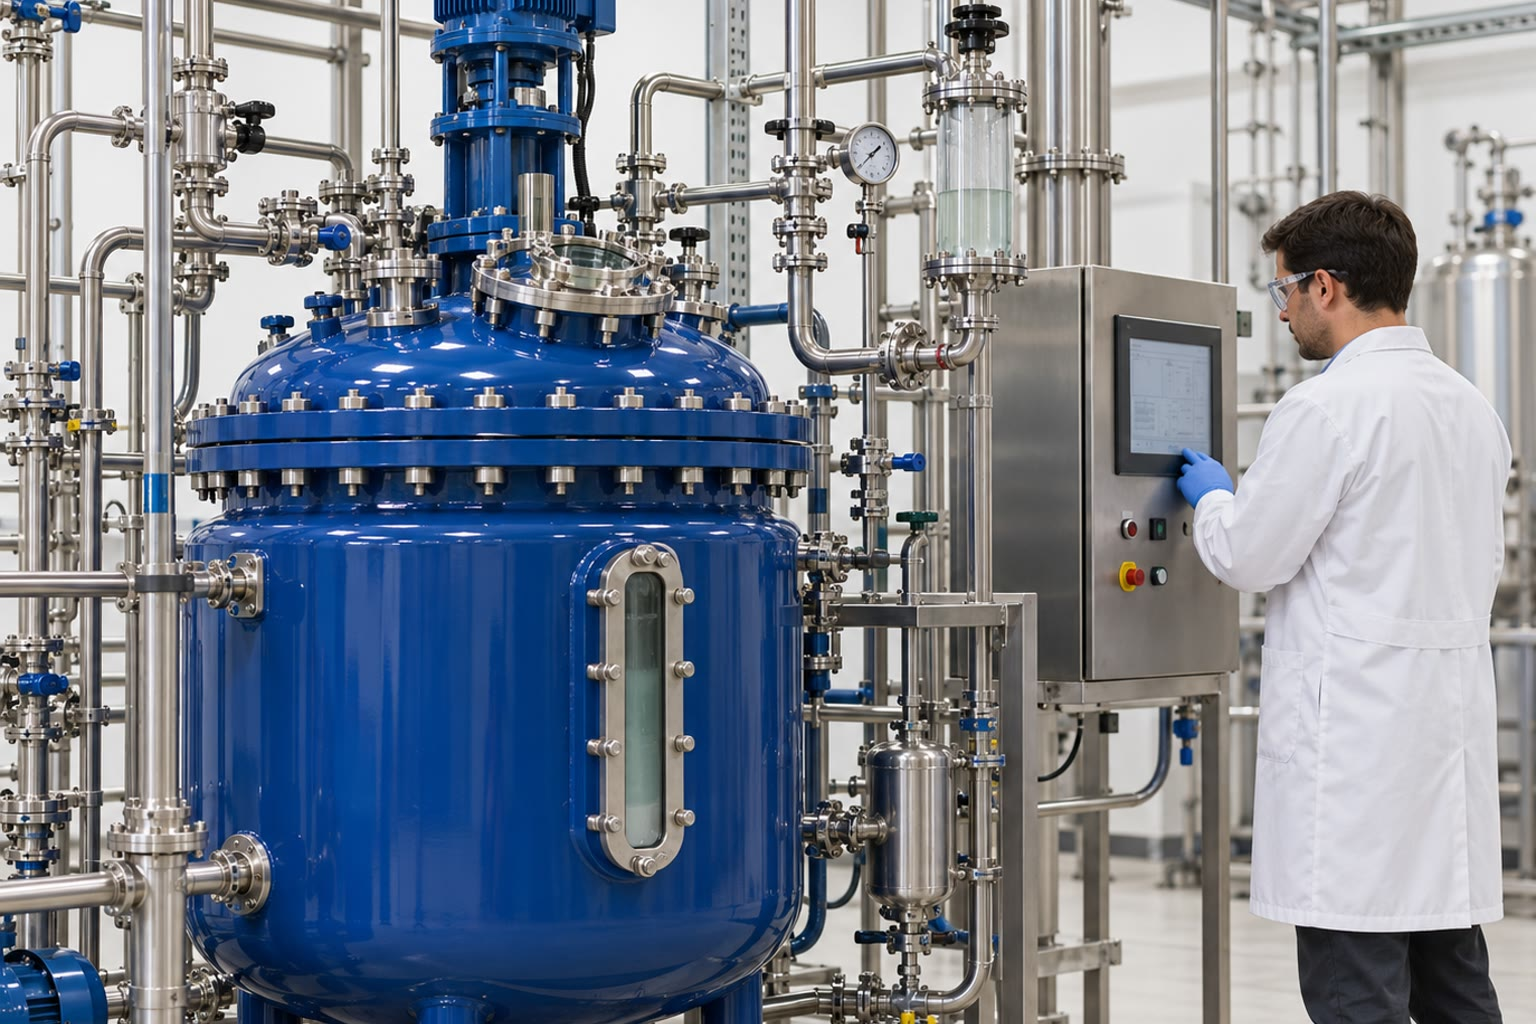
\includegraphics[width=0.62\linewidth]{images/book3/ai/b2-20-pilot-plant.jpg}

{\small 工艺化学的中试装置：搪玻璃钢反应釜，
其中催化偶联反应在投产前由烧瓶规模放大而来。}
\end{omfigure}

\section{有机金属配合物的语言}

有机金属配合物的计数方法与\cref{met:b2:coordination-complexes:electron-count}相同，
只是配体稍多：氢负离子 \ce{H-} 与烷基或芳基阴离子 \ce{R-}
各提供两个电子，氧化数均计为 $-1$；\ce{CO}、膦类 \ce{PR3} 与
$\eta^2$-烯烃提供两个电子，氧化数计为 0；卤离子 \ce{X-}
提供两个电子，氧化数计为 $-1$。

\begin{definition}[配位不饱和配合物]\label{def:b2:catalytic-cycles:unsaturated}
称\emph{配位不饱和配合物}\index{配位不饱和配合物}
为价电子数少于 18（常为 16）、能再结合一个配体的配合物，
它具有一个\emph{空配位点}\index{空配位点}，即\omterm{def:b2:coordination-complexes:coordination-sphere}{配位层}中空出的、
可接受一个两电子给体的位置。
\end{definition}

平面正方形的 $d^8$ 配合物，如铑(I)、铱(I)、钯(II)和
铂(II)的配合物都是 16 电子配合物；钯(0)的双膦配合物 \ce{PdL2} 则为 14 电子。
这类配合物是多数\omterm{def:b2:catalytic-cycles:cycle}{催化循环}中的活性物种。

\begin{method}[有机金属配合物的计数]\label{met:b2:catalytic-cycles:count-organometallic}
\begin{enumerate}
  \item 列出配体：阴离子型（\ce{H-}、\ce{R-}、\ce{X-}、\ce{C5H5-}）和
        中性配体（\ce{CO}、\ce{PR3}、烯烃、溶剂）。
  \item 氧化数 = 配合物的电荷 $-$ 阴离子配体电荷之和。
  \item $n = g -$ 氧化数；电子计数 = $n + 2 \times$（两电子给体的个数）
        $+$ 每个 $\eta^5$-\ce{C5H5-} 计 6 个电子。
  \item 配位数 = 被占据的配位位点数。
\end{enumerate}
\end{method}

\section{配体交换、氧化加成、还原消除}

\begin{definition}[配体交换]\label{def:b2:catalytic-cycles:ligand-exchange}
称\emph{配体交换}\index{配体交换}为一类基元反应，其中\omterm{def:b2:coordination-complexes:coordination-sphere}{配位层}的
一个配体被另一配体取代；它既不改变氧化数，
总体上也不改变电子计数。其机理在本科三年级分册中讨论。
\end{definition}

\begin{definition}[氧化加成与还原消除]\label{def:b2:catalytic-cycles:oxidative-addition}
在\emph{氧化加成}\index{氧化加成}中，分子 A--B 加到一个
金属中心上，断裂其自身的 A--B 键，形成 M--A 与 M--B 键。
\emph{还原消除}\index{还原消除}为其逆步骤：互呈顺式的两个配体 A 与 B
结合为 A--B，并脱离金属。
\end{definition}

\begin{proposition}[氧化加成的计数]\label{prop:b2:catalytic-cycles:oa}
\omterm{def:b2:catalytic-cycles:oxidative-addition}{氧化加成}使金属的氧化数升高 2，其\omterm{def:b2:coordination-complexes:electron-count}{价电子计数}
增加 2，配位数增加 2；\omterm{def:b2:catalytic-cycles:oxidative-addition}{还原消除}则使三者各降低 2。
\end{proposition}

\begin{proof}
A 与 B 结合后按阴离子计数（\ce{H-}、\ce{R-}、\ce{X-}）：两个新增
阴离子配体使氧化数升高 2，$n$ 降低 2；它们提供两对，即 $+4$
个电子；计数变化为 $-2 + 4 = +2$。两个配位位点新被占据。
逆过程使每一项变化都反向。
\end{proof}

\begin{example}[瓦斯卡配合物]\label{ex:b2:catalytic-cycles:vaska}
\ce{[IrCl(CO)(PPh3)2]}，平面正方形：铱(I)，$d^8$，16 电子，四配位。
它与氢分子加成，得 \ce{[IrH2Cl(CO)(PPh3)2]}，铱(III)，$d^6$，18 电子，八面体，
两个氢负离子呈顺式。
\end{example}

\section{插入、消除、转金属化}

\begin{definition}[插入与 $\beta$-氢消除]\label{def:b2:catalytic-cycles:insertion}
在\emph{迁移插入}\index{迁移插入}中，与金属相连的不饱和配体
（烯烃、\ce{CO}）插入顺式的 M--H 或 M--C 键中：\ce{M-H} 与一个
烯烃给出烷基 \ce{M-CH2-CH2-H}；\ce{M-R} 与 \ce{CO} 给出酰基 \ce{M-C(=O)R}。
\emph{$\beta$-氢消除}\index{$\beta$-氢消除}
是烯烃插入的逆过程：即位于相对金属为 $\beta$ 位的碳上的氢
转移到金属上，同时释放出一个烯烃。
\end{definition}

\begin{proposition}[插入的计数]\label{prop:b2:catalytic-cycles:insertion}
\omterm{def:b2:catalytic-cycles:insertion}{迁移插入}保持氧化数不变，使电子计数降低 2
（释放出一个配位位点）；$\beta$-氢消除则使计数升高 2。
\end{proposition}

\begin{proof}
插入前：\ce{H-}（或 \ce{R-}，阴离子）与烯烃（中性），共两个配体、四个电子。
插入后：一个烷基（阴离子），两个电子。阴离子电荷未变，故
氧化数不变；电子减少两个，配位位点也减少一个。
\end{proof}

\begin{proposition}[$\beta$-氢消除的条件]\label{prop:b2:catalytic-cycles:beta-h}
金属烷基发生 $\beta$-氢消除，仅当烷基的 $\beta$ 碳上带有氢，
且金属上有与烷基顺式的空配位位点。
\end{proposition}

\begin{proof}[论证]
该步骤经过一个四元结构 M--C$_\alpha$--C$_\beta$--H，其中
氢原子转移至金属上。这需要有这个氢原子，以及烷基旁边的一个空位置来接收它。
甲基、苄基、新戊基和芳基没有能够到达金属的 $\beta$ 氢，
因而对此反应稳定。
\end{proof}

\begin{definition}[转金属化]\label{def:b2:catalytic-cycles:transmetalation}
称\emph{转金属化}\index{转金属化}为将有机基团从一种金属
（或类金属：硼、锌、锡）转移到另一种金属上，通常同时换出一个卤化物。
\end{definition}

\begin{omfigure}
\begin{tikzpicture}[font=\small, >={Stealth}]
  \tikzset{omstepar/.style={->, thick}}
  \foreach \y/\l/\r/\top/\bot/\rev in {
      0/{$\mathrm{L}_n\mathrm{M}$}/{$\mathrm{L}_n\mathrm{M(A)(B)}$}/{+ A--B}/{氧化加成}/{还原消除},
      -1.5/{$\mathrm{L}_n\mathrm{M(H)(CH_2{=}CH_2)}$}/{$\mathrm{L}_n\mathrm{M{-}CH_2CH_3}$}/{}/{迁移插入}/{$\beta$-氢消除},
      -3.0/{$\mathrm{L}_n\mathrm{M(X)(R)}$}/{$\mathrm{L}_n\mathrm{M(R)(R')}$}/{+ R$'$--[B], $-$ X--[B]}/{转金属化}/{},
      -4.5/{$\mathrm{L}_n\mathrm{M(X)}$}/{$\mathrm{L}_n\mathrm{M(X)(L')}$}/{+ L$'$}/{配体交换或配位}/{}} {
    \node[cyclenode, anchor=east] (l) at (0,\y) {\l};
    \node[cyclenode, anchor=west] (r) at (5.2,\y) {\r};
    \draw[omstepar] ($(l.east)+(0.1,0.08)$) -- ($(r.west)+(-0.1,0.08)$) node[midway, above, font=\scriptsize] {\top};
    \node[font=\scriptsize, anchor=north] at (2.6,\y-0.02) {\bot};
    \node[font=\scriptsize, black!55, anchor=west] at (5.2,\y-0.5) {\rev};
  }
\end{tikzpicture}

{\small 有机金属催化的基元反应。\omterm{def:b2:catalytic-cycles:oxidative-addition}{氧化加成}：氧化
数、电子计数与配位数均增加 $+2$；\omterm{def:b2:catalytic-cycles:oxidative-addition}{还原消除}：$-2$。\omterm{def:b2:catalytic-cycles:insertion}{迁移
插入}：电子计数 $-2$，氧化数不变；$\beta$-氢消除
为其逆过程。\omterm{def:b2:catalytic-cycles:transmetalation}{转金属化}：有机基团从硼、锌或锡转移到金属上。}
\end{omfigure}

\section{读懂催化循环}

\begin{definition}[催化循环]\label{def:b2:catalytic-cycles:cycle}
称\emph{催化循环}\index{催化循环}为由基元反应组成的闭合序列，
它消耗试剂、释放生成物，并使其第一个配合物再生。
加入反应体系、并转化为循环第一个配合物的化合物，称为
\emph{预催化剂}\index{预催化剂}。\emph{转化数}\index{转化数}
（TON）是每单位催化剂生成的产物的量；\emph{转化
频率}\index{转化频率}（TOF）是单位时间内的转化数。
\end{definition}

\begin{proposition}[总反应方程]\label{prop:b2:catalytic-cycles:cycle-sum}
\omterm{def:b2:catalytic-cycles:cycle}{催化循环}各基元反应之和即为被催化反应的方程式：
每个金属配合物既作为生成物出现一次，又作为反应物出现一次，相互抵消。
\end{proposition}

\begin{proof}
循环是闭合的，每个中间体由一步生成、又由下一步消耗；
将各步相加时，这些物种在两侧出现并相互抵消，
剩下的便是从外部加入的试剂和离开体系的生成物。
\end{proof}

\begin{method}[读懂催化循环]\label{met:b2:catalytic-cycles:read-cycle}
\begin{enumerate}
  \item 对每个配合物，计算其氧化数、电子计数与
        配位数。
  \item 根据变化为各步骤命名（$+2/+2/+2$：\omterm{def:b2:catalytic-cycles:oxidative-addition}{氧化加成}；氧化数不变而电子计数 $-2$：
        插入；依此类推）。
  \item 检查没有配合物超过 18 个电子，且需要\omterm{def:b2:catalytic-cycles:unsaturated}{空配位点}的步骤
        从\omterm{def:b2:catalytic-cycles:unsaturated}{配位不饱和配合物}出发。
  \item 将各步相加：其和应为总反应方程。
\end{enumerate}
\end{method}

\begin{omfigure}
\begin{tikzpicture}[font=\small, >={Stealth}]
  \node[cyclenode] (n1) at (90:2.3) {\ce{[RhCl(PPh3)2]}\\ Rh(I)，14 电子};
  \node[cyclenode] (n2) at (0:3.4) {\ce{[RhH2Cl(PPh3)2]}\\ Rh(III)，16 电子};
  \node[cyclenode] (n3) at (270:2.3) {\ce{[RhH2Cl(PPh3)2(RCH=CH2)]}\\ Rh(III)，18 电子};
  \node[cyclenode] (n4) at (180:3.4) {\ce{[RhH(CH2CH2R)Cl(PPh3)2]}\\ Rh(III)，16 电子};
  \draw[cyclearc] (n1) to[bend left=20] node[cyclelabel, below left] {氧化 \\ 加成} (n2);
  \draw[cyclearc] (n2) to[bend left=20] node[cyclelabel, left=12pt] {烯烃 \\ 配位} (n3);
  \draw[cyclearc] (n3) to[bend left=20] node[cyclelabel, above right] {迁移 \\ 插入} (n4);
  \draw[cyclearc] (n4) to[bend left=20] node[cyclelabel, below right] {还原 \\ 消除} (n1);
  \draw[cyclein] (4.6,2.3) node[right] {\ce{H2}} -- (2.6,1.75);
  \draw[cyclein] (4.6,-2.3) node[right] {烯烃} -- (2.6,-1.75);
  \draw[cycleout] (-2.6,1.75) -- (-4.6,2.3) node[left] {烷烃};
  \node[font=\scriptsize, align=center, black!60] at (0,-0.05) {预催化剂 \\ \ce{[RhCl(PPh3)3]}\\ 失去一个 \ce{PPh3}};
\end{tikzpicture}

{\small 威尔金森催化剂作用下烯烃的催化氢化（简化示意，省略膦配体与溶剂的
交换）。四步之和为 $\ce{RCH=CH2 + H2 -> RCH2CH3}$；
铑配合物相互抵消。}
\end{omfigure}

\begin{omfigure}
\begin{tikzpicture}[font=\small, >={Stealth}]
  \node[cyclenode] (s1) at (90:2.3) {\ce{PdL2}\\ Pd(0)，14 电子};
  \node[cyclenode] (s2) at (0:3.4) {\ce{[ArPd(Br)L2]}\\ Pd(II)，16 电子};
  \node[cyclenode] (s3) at (270:2.3) {$[\mathrm{ArPd(Ar')L_2}]$\\ Pd(II)，16 电子};
  \draw[cyclearc] (s1) to[bend left=25] node[cyclelabel, below left] {氧化 \\ 加成} (s2);
  \draw[cyclearc] (s2) to[bend left=25] node[cyclelabel, above left] {转金属化} (s3);
  \draw[cyclearc] (s3) to[bend left=35] node[cyclelabel, right] {还原 \\ 消除} (s1);
  \draw[cyclein] (4.8,2.2) node[right] {\ce{Ar-Br}} -- (2.6,1.6);
  \draw[cyclein] (5.4,-0.9) node[right, align=left] {$\mathrm{Ar'B(OH)_2}$\\ + 碱} -- (3.3,-1.2);
  \draw[cycleout] (2.3,-2.0) -- (4.4,-2.9) node[right] {\ce{Br-}, \ce{B(OH)3}};
  \draw[cycleout] (-1.75,-0.4) -- (-4.2,-0.4) node[left] {$\mathrm{Ar{-}Ar'}$};
\end{tikzpicture}

{\small 铃木偶联的简化示意。钯(0)加入芳基溴；碱
将硼酸转化为硼酸根，后者把其芳基转移到钯上；
两个顺式的芳基消除为联芳基，使钯(0)再生。}
\end{omfigure}

在赫克反应中，经\omterm{def:b2:catalytic-cycles:oxidative-addition}{氧化加成}形成的芳基–钯配合物与一个烯烃结合，而不是与硼酸根结合；
\omterm{def:b2:catalytic-cycles:insertion}{迁移插入}使芳基连到烯烃上，
随后 $\beta$-氢消除释放出取代烯烃（通常为反式异构体）和一个氢化钯，
氢化钯再被碱脱去 \ce{HBr}，使钯(0)再生。

加氢甲酰化是 \ce{H2} 与 \ce{CO} 对烯烃的加成，生成醛，
在钴或铑氢化物上进行，依次为烯烃插入、\ce{CO} 插入
金属–烷基键、\ce{H2} 的\omterm{def:b2:catalytic-cycles:oxidative-addition}{氧化加成}以及醛的\omterm{def:b2:catalytic-cycles:oxidative-addition}{还原消除}。
第一步插入的方向决定产物：金属位于末端碳上时得直链醛，
位于内侧碳上时得支链醛；
体积大的膦配体有利于生成直链产物。

\begin{history}[交叉偶联]
\begin{minipage}[t]{0.36\linewidth}
\vspace{0pt}
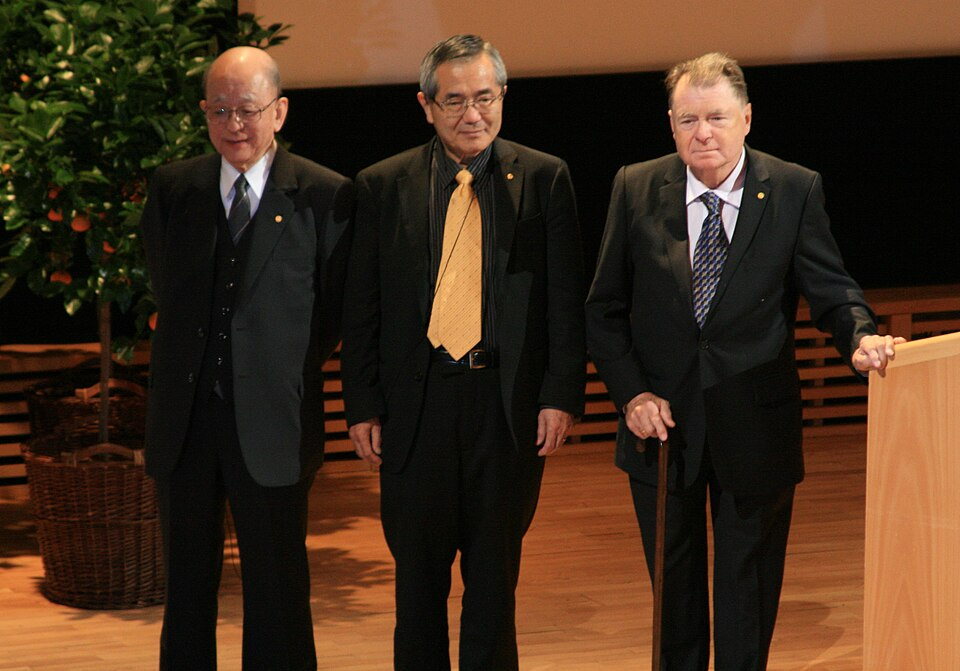
\includegraphics[width=\linewidth]{images/book3/nobel-2010.jpg}
\end{minipage}\hfill
\begin{minipage}[t]{0.6\linewidth}
\vspace{0pt}
以钯为催化剂，芳基和乙烯基卤代物与烯烃的偶联（理查德·赫克，1968 年起）、
与有机锌试剂的偶联（根岸英一，1977 年）以及与有机硼化合物的偶联（铃木章，1979 年），
使两个碳骨架的连接变得常规化；如今它们是药物与材料合成中最常用的反应之一。
诺贝尔化学奖于 2010 年授予了这三位科学家。
（照片：从左到右依次为铃木章、根岸英一和理查德·赫克，
2010 年；BloodIce，CC BY-SA 4.0，维基共享资源。）
\end{minipage}
\end{history}

\begin{proposition}[转化数]\label{prop:b2:catalytic-cycles:tof}
设 $n_P$ 为时间 $t$ 内由物质的量为 $n_{\text{cat}}$ 的催化剂生成的产物的量，
则 $\mathrm{TON} = n_P/n_{\text{cat}}$，平均\omterm{def:b2:catalytic-cycles:cycle}{转化频率}为 $\mathrm{TOF} =
\mathrm{TON}/t$。
\end{proposition}

\begin{proof}
循环每转动一次，每个金属原子生成一个产物分子；每个原子平均转动的次数为
$n_P/n_{\text{cat}}$，
转动速率即为单位时间内的这一次数。
\end{proof}

\begin{safety}{\ghs[5mm]{GHS05}\,\ghs[5mm]{GHS07}\,\ghs[5mm]{GHS09}}
乙酸钯(II)对眼睛有腐蚀性，对水生生物有毒；
三苯基膦有害，并且是致敏物。称量应在通风橱中进行，
钯的残留物须收集以便回收，切勿倒入下水道。
% ledger: ghs:Pd-acetate, ghs:PPh3, ghs:phenylboronic-acid, ghs:4-bromotoluene
\end{safety}

\section{练习}

\begin{exercise}[$\star$]\label{exo:b2:catalytic-cycles:1}
写出瓦斯卡配合物 \ce{[IrCl(CO)(PPh3)2]} 的氧化态、$d^n$ 和电子计数，
并给出其加入 \ce{H2} 前后的数值。
\end{exercise}

\begin{exercise}[$\star$]\label{exo:b2:catalytic-cycles:2}
指出各步骤的类型：\ce{[PtCl2(CH3)2(PR3)2] -> [PtCl2(PR3)2] + C2H6}；\ce{[Pd(Ph)Br(PR3)2] +
CH2=CH2 -> [Pd(CH2CH2Ph)Br(PR3)] + PR3}。
\end{exercise}

\begin{exercise}[$\star$]\label{exo:b2:catalytic-cycles:3}
某反应使用 \qty{0.020}{mmol} 催化剂，得到 \qty{15.0}{mmol} 产物，
所用时间为 \qty{3.0}{h}。计算 TON 和平均 TOF。
\end{exercise}

\begin{exercise}[$\star$]\label{exo:b2:catalytic-cycles:4}
将铃木循环的三个步骤相加，并检验钯是否被消去。
\end{exercise}

\begin{exercise}[$\star\star$]\label{exo:b2:catalytic-cycles:5}
下列烷基钯配合物中，哪些能够发生 $\beta$-氢消除：
\ce{Pd-CH3}、\ce{Pd-CH2CH3}、\ce{Pd-CH2C(CH3)3}、\ce{Pd-CH2Ph}、\ce{Pd-CH(CH3)2}？
\end{exercise}

\begin{exercise}[$\star\star$]\label{exo:b2:catalytic-cycles:6}
预测碘苯与丙烯酸甲酯发生赫克反应的产物，
并写出其构型。
\end{exercise}

\begin{exercise}[$\star\star$]\label{exo:b2:catalytic-cycles:7}
写出丙烯加氢甲酰化生成的直链醛和支链醛，
并说明各由哪一步插入得到。
\end{exercise}

\begin{exercise}[$\star\star$]\label{exo:b2:catalytic-cycles:8}
为什么 \ce{[RhCl(PPh3)3]} 只有在失去一个膦配体后才能加成 \ce{H2}，
而 \ce{[RhCl(PPh3)2]} 则可立即加成？
\end{exercise}

\begin{exercise}[$\star\star$]\label{exo:b2:catalytic-cycles:9}
在铃木偶联中，为什么需要碱？它对硼酸起什么作用？
\end{exercise}

\begin{exercise}[$\star\star\star$]\label{exo:b2:catalytic-cycles:10}
某一拟定的循环用于 $d^8$ 配合物 \ce{ML3X}（16 e）上烯烃的氢化，
首先烯烃与之结合生成 20 电子配合物，随后发生\omterm{def:b2:catalytic-cycles:oxidative-addition}{氧化加成}，
加成试剂为 \ce{H2}。找出其中的错误并更正步骤顺序。
\end{exercise}

\begin{exercise}[$\star\star\star$]\label{exo:b2:catalytic-cycles:11}
催化反应产物的量按 $n_P(t) = n_{\max}(1 - \mathrm e^{-t/\tau})$ 增长，
其中 $n_{\max} = \qty{10.0}{mmol}$，$\tau = \qty{40}{min}$，催化剂的量为 \qty{0.010}{mmol}，
（练习数据）。计算初始 TOF 与最终 TON。
\end{exercise}

\begin{exercise}[$\star\star\star$]\label{exo:b2:catalytic-cycles:12}
设计一个交叉偶联反应以制备 4-甲氧基联苯，选择卤代物和硼酸，
并写出其循环。
\end{exercise}

\section{问题：阅读铃木循环}

\begin{problem}[{周末问题——预催化剂与活性零价钯，
铃木偶联的氧化加成、转金属化与还原消除，
产率与转化数，以及副反应}]
\label{pb:b2:catalytic-cycles:1}
反应体系（练习数据）：\qty{10.0}{mmol} 4-溴甲苯，\qty{12.0}{mmol}
苯硼酸，\qty{20}{mmol} 碳酸钾，\qty{0.050}{mmol}
乙酸钯(II)，\qty{0.10}{mmol} 三苯基膦，于甲苯、乙醇和
水的混合溶剂中，氮气保护下加热；分离产物：\qty{1.51}{g} 4-甲基联苯。摩尔
质量（\unit{g/mol}）：4-溴甲苯 171.04，苯硼酸 121.93，4-甲基联苯
168.24，乙酸钯(II) 224.51。
% ledger: aw:C, aw:H, aw:Br, aw:B, aw:O, aw:Pd

\medskip
\noindent\textbf{第一部分——催化剂。}
\begin{enumerate}
  \item 写出乙酸钯(II)中钯的氧化态及其 $d^n$ 构型。
  \item 烧瓶中它被还原为 \ce{Pd(PPh3)2}，写出其氧化态、$d^n$
        及电子计数。
  \item 该配合物为何是配位不饱和的？
  \item 反应为何要在氮气中进行？
  \item 过量三苯基膦起什么作用？
  \item 乙酸钯(II)是催化剂还是\omterm{def:b2:catalytic-cycles:cycle}{预催化剂}？
\end{enumerate}

\medskip
\noindent\textbf{第二部分——各步反应。}
\begin{enumerate}[resume]
  \item 写出 4-溴甲苯的\omterm{def:b2:catalytic-cycles:oxidative-addition}{氧化加成}，并计算产物的电子计数。
  \item 碳酸根对苯硼酸起什么作用？
  \item 写出\omterm{def:b2:catalytic-cycles:transmetalation}{转金属化}过程。
  \item 为何在下一步之前两个芳基必须处于顺式？
  \item 写出\omterm{def:b2:catalytic-cycles:oxidative-addition}{还原消除}过程，并计算生成的钯物种的电子计数。
  \item 将三步反应相加。
\end{enumerate}

\medskip
\noindent\textbf{第三部分——产率与\omterm{def:b2:catalytic-cycles:cycle}{转化数}。}
\begin{enumerate}[resume]
  \item 哪种试剂是限量试剂？
  \item 计算分离得到的产物的量。
  \item 计算产率。
  \item 以溴代物为基准，计算催化剂用量，以 mol~\% 表示。
  \item 计算钯的\omterm{def:b2:catalytic-cycles:cycle}{转化数}。
  \item 反应进行了 \qty{4.0}{h}。计算每小时的平均\omterm{def:b2:catalytic-cycles:cycle}{转化频率}。
\end{enumerate}

\medskip
\noindent\textbf{第四部分——副反应。}
\begin{enumerate}[resume]
  \item 检出了一些联苯 \ce{Ph-Ph}。推测其生成途径。
  \item 为何此处不可能发生 $\beta$-氢消除？
  \item 芳基氯化物的反应远比溴代物慢。哪一步受到阻碍？
  \item 反应结束时钯发生了什么变化？为何能被回收？
  \item 为何使用少量过量的硼酸？
  \item 写出本次反应中钯的\omterm{def:b2:catalytic-cycles:cycle}{转化数}。
\end{enumerate}
\end{problem}
